\section{Les différentes attaques}
Une fois en possession des diverses informations, il existe un
très grand nombre d'attaques différentes pour retrouver le message
clair ou la clé utilisée pendant le chiffrement. Voyons les
attaques les plus utilisées.

\subsection{L'analyse des fréquences}
Exposée pour la première fois par Al-Kindi au IX\ieme~ siècle,
l'analyse fréquentielle permet de déchiffrer des chiffrements
simples. Dans le cas d'une substitution, les
caractères sont représentés par autre chose, mais leur fréquences
d'apparition ne change pas, on peut donc alors facilement
retrouver le message initial, connaissant les fréquences
normale d'apparition des caractères dans la langue du message.

L'analyse des fréquence ne se limite pas aux lettres
individuelles, l'analyse des bigrammes peut aussi être très
pratique.
\\

On peut via cette méthode aussi trouver la langue dans laquelle le
message est écrit, car chaque langue possède une fréquence
d'apparitions des lettres unique (voir la figure \ref{fig:Frequences}).

Bien évidemment, la fréquence d'apparition des lettres peut varier
au sein d'une même langue selon certains critères (par exemple un
message d'origine militaire risque de contenir beaucoup
d'abréviations).

\begin{figure}[h]
  \centering
    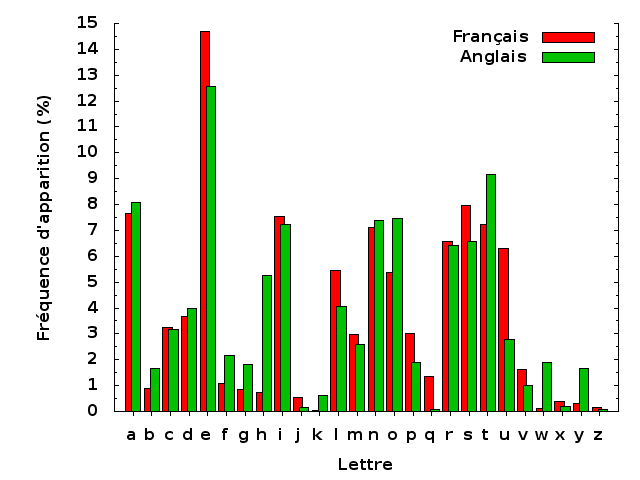
\includegraphics[width=0.9\textwidth]{plot/Frequences.png}
    \caption{Fréquences d'apparition des lettres en français et en
anglais}
  \label{fig:Frequences}
\end{figure}
\subsection{L'indice de coïncidence}
\subsection{L'attaque par mot probable}

\subsection*{Application : cassage d'un cryptogramme proposé par
le FBI}
Pour mettre en pratique l'analyse des fréquences et l'attaque par
mot probable, nous allons
casser un message chiffré\footnote{Disponible sur
\url{http://www.fbi.gov/page2/nov07/code112107.html}}, 
proposé par le FBI sur leur site fin
octobre 2007 (conçus par leurs cryptanalystes « just for fun »)
\\
Le cryptogramme est donc « PIKODENHFENJIKM! YIH QELB GDISBK NQB
PICB. OI NI AGJ.OIL/PICB.QNT MI WB SKIW, EKC UFBEMB PIKMJCBD E
PEDBBD WJNQ NQB AGJ. »

À première vue, le cryptogramme à tout l'air d'une substitution
monoalphabétique, du fait de la présence d'espaces et de
ponctuation.
Avant tout, essayons de trouver des éléments spéciaux dans le
cryptogramme. On remarque assez vite un E seul vers la fin, ce qui
a beaucoup de chance de correspondre avec la lettre A (« a » étant
le seul mot composé d'une lettre en anglais), ainsi que le «
AGJ.OIL/PICB.QNT », qui ressemble à une URL (sans le préfixe
\emph{www}). Comme ce code est proposé par le site
\url{www.fbi.gov}, on se doute bien que c'est cette même URL.
\\

Faisons ensuite une analyse des fréquences ; les lettres
apparaissant le plus souvent dans le cryptogramme sont I et B (12
fois), N et E (7 fois), et K (6 fois).
Nous savons déjà que I correspond à O en clair, et E correspond à
A. En regardant les fréquences moyenne d'apparition des lettres en
anglais, la lettre apparaissant le plus est le E, qui devrait
correspondre à B ici, suivie de la lettre T, qui correspond alors
sûrement à N, et enfin (après A et O, que nous connaissons déjà),
viens la lettre N, qui correspond donc sûrement à K ici.
\\

Nous connaissons alors déjà quelques correspondances entre lettres
claires et lettres chiffrées : \\
\begin{center}
  \begin{tabular}{c|c}
    Lettre claire & Lettre chiffrée \\
    \hline
    A & E \\
    F & A \\
    B & G \\
    I & J \\
    G & O \\
    O & I \\
    V & L \\
    E & B \\
    T & N \\
    N & K
  \end{tabular}
\end{center}

On pourrait encore essayer de trouver plus de lettres via
l'analyse des fréquence des lettres et des bigrammes présent dans
le cryptogramme.
\\

La suite consiste à écrire le message avec les lettres que nous
connaissons déjà, et à essayer de trouver les lettres manquantes.

Ainsi, le premier mot serait « \_ONG\_AT\_\_ATION\_! », et on trouve
assez rapidement que ce mot est « CONGRATULATIONS! », ce qui nous
permet de connaître encore 5 lettres de plus.

Il suffit alors de continuer ainsi de suite jusqu'à avoir
déchiffré le message en entier, dans ce cas ci, le message clair
est « CONGRATULATIONS! YOU HAVE BROKEN THE CODE. GO TO
FBI.GOV/CODE.HTM SO WE KNOW, AND PLEASE CONSIDER A CAREER WITH THE
FBI »
